% !TEX encoding = UTF-8 Unicode
%!TEX root = thesis.tex
% !TEX spellcheck = en-US
%%=========================================
\documentclass[thesis.tex]{subfiles}
\begin{document}
	\chapter[Conclusions]{Conclusions, Discussion, and Recommendations for Further Work}
	\label{ch:conclusions}
	Having reached the end of this expos\'e, as formality would dictate, the time has come to sum up the ideas contain in the previous chapters and paragraphs. At first, a succinct summary is put forth in section \ref{sec:summary_and_conclusions}, followed by a thorough discussion of the main results in section \ref{sec:discussion}, without leaving out its limitations. As every scientific work is build upon previous ideas, to strengthen and extend the results formerly formulated, section \ref{sec:recommendations_for_further_work}, presents a list of recommendations.
	%%This is the last chapter
	%In this final chapter you should sum up what you have done and which results you have got. 
	%You should also discuss your findings, and give recommendations for further work.
	
	%%=========================================
	\section{Summary and Conclusions}
	\label{sec:summary_and_conclusions}
	%Here, you present a brief summary of your work and list the main results you have got. 
	%You should give comments to each of the objectives in Chapter 1 and state whether or not you have met the objective. 
	%If you have not met the objective, you should explain why (e.g., data not available, too difficult).
	%
	%This section is similar to the Summary and Conclusions in the beginning of your report, but more detailed---referring to the the various sections in the report.
	The industrial revolution had set up a chain of events, that forged efficiency in all economical sectors, and consequently led to improvements, in nearly all physical and material aspects of human live. All this progress would not have been possible without machines. However, they are prone to failure, and must be monitor and maintain, to avoid unexpected and catastrophic breakdown. To mitigate such events, most machines are equipped with an array of sensors, collecting continuously data. A myriad of methods and algorithms make it possible to analyze the data generated, in order to detect as early as possible any sign of failure, and take necessary actions.
	\justify
	In this thesis, we posited two new methods for bearings faults detection, which represent more than 40 $\%$ of all deterioration in rotating machines. By facilitating rotational movements, bearings are critical part of nearly all rotating equipment. They are continually subjected to extensive load, thereby must be closely kept under observation. The most widely applied method for bearing fault detection, is a Fourier transform based methodology. In the latter, a bearing vibration signal is filtered and decomposed into a spectrum of frequencies. For a bearing, the failure frequency is derived from its geometrical components and the rotational speed of the machine on which it is mounted. Once the failure frequency is known, it suffices to search for it in the frequency spectrum, derived from the Fourier transform of a bearing vibration signal. 
	%To set a reference method, the Fourier transformed based method was introduced, followed by two new methods that extend the limitations of the latter.
	\justify
	In Chapter 2, we introduced the Fourier transform (FT) based method, which was later applied to a case study.
	In the latter, a machine housing four bearings and rotating at 2000 revolutions per minute, was run to failure.
	At the end of the experiment, one of the bearing had a sever damage in its outer layer. This fault is know as ball pass frequency outer race defect. A sensor recording the vibration movement was placed on each bearing, in order to monitor any potential damages. This resulted in collecting 984 samples, where each sample containing 20 480 data points, was saved every 10 minutes.
	\justify
	Each sample, which we refer to as signal, was subjected to three filters: A band, high and low pass filter, to remove unwanted noise and frequencies. The resulting signal was decomposed into its frequency spectrum. The latter contains all frequencies at which the bearing is vibrating, including the ball pass outer race frequency, previously mentioned.
	The ball pass frequency outer race defect, (which is the defect frequency) is derived from the bearing physical characteristics, as well as the rotation speed of the motor. Conceptually, a bearing with a defect, will produce a sub-signal, which is a sinusoidal function with amplitude and frequency corresponding to the ball pass frequency outer race defect. After estimating that frequency, a search is performed in the frequency spectrum. Once it is found, we just keep track of the amplitude of the sub-signal it produced.
	\justify
	By applying the Fourier transform based method, we were able to detect the onset of failure in the bearings outer race and track its evolution over time. However, when using the Fourier transform method, the dependency of failure frequency on the rotational speed of the motor, can incur difficulties for continuously varying rotational speed or even poor data quality. In addition, the Fourier transform method is not well equipped in dealing with non-linear and non-stationary signals. The assumption of an a-priory trigonometrical basis, which are globally define, limits the FT based method in capturing local phenomenon such high frequency pulses emitted by a crack in bearings.
	\justify
	To circumvent some of the short coming of the Fourier transform, the Hilbert Huang transform (HHT) was introduced in Chapter 3.
	This method adaptively decomposes a signal into sub-signals called intrinsic mode functions (IMFs), by a process called empirical mode decomposition (EMD). It uses local properties (extrema, envelop) and statistical estimator (mean) to iteratively	\say{siffer} a signal into its sub-components. This allows decomposing non-stationary and nonlinear data with ease. In addition local phenomenon such as high frequency pulses emitted by cracks in bearing can be detected by this method. By applying the EMD coupled with a robust seasonal trend decomposition method, it was possible to extract high frequency, short duration pulses emitted by a crack located in the outer ring of a bearing.
	\justify
	In chapter 4, we introduced a method that uses the duo wavelet transform-support vector machine, to monitor and detect outer race defect for a system of four bearings attached to a motor. The new methodology consists of three stages: In the first stage, the wavelet transform decomposes a bearing vibration signal into two additional signals. They were called frequency and temporal features. The former and the latter encode frequency and temporal information, and together form the temporal-frequency feature space. In the second stage, the interquartile range (IQR) of the frequency and temporal feature are estimated, for successive vibration samples measured in time. The IQR which is a robust statistical estimator, measures the bulk of variability, and quantifies the health of a sample. A higher IQR implies an \say{unhealthy} sample. In doing so, we obtained several points in the temporal-frequency feature space.
	\justify
	In the last stage, a one class support vector machine (SVM) classifier was applied to the set of points generated in the temporal-frequency feature space. The SVM, which is a linear classification algorithm, was able to set a boundary between \say{healthy} and \say{unhealthy} samples.
	This new methodology was able to detect earlier the onset of failure for one of the bearings which was severely affected by a defect in the outer race.
	
	
	
	%%=========================================
	\section{Discussion}
	\label{sec:discussion}
	The contribution of this thesis rests on two methods: Hilbert Huang transform coupled with the seasonal trend base on Loess (HHT-STL) and wavelet transform coupled with support vector machine (WT-SVM). Both methods are simple and require less transformation as opposed to the Fourier transform based method. In the latter the input signal needs to be filter by a band, high and low pass filter, before being decomposed into it frequency spectrum. Moreover, detecting fault requires the knowledge of the frequency spectrum which depends on bearings physical characteristics and rotation speed on the motor housing the bearings. In contrast, the two new methods are direct, and only rely on the signal.
	\justify
	The HHT-STL method was introduced as a tool to extract high frequency short duration pulses. It is used as a proof of concept. Once pulses are extracted, their frequency and amplitude represent the failure characteristics of a bearing. To monitor a bearing we just need to track the amplitude of a pulse. However, at this stage, for this method to be useful in application, two questions need to be answered 
	\justify
	How to choose the correct intrinsic mode function ?. Does the amplitude and the frequency of the pulse corresponds to the failure frequency on a bearing? 
	The first question is related to the fact that the Hilbert Huang transform generates many intrinsic mode functions (IMFs). When a bearing mounted on a motor vibrates, the resulting signal encompasses multiple sub-signals that correspond to other components on the motor, including the bearing it self. This include but not limited to: the rotating motor shaft, other bearings, the motor cage, the belts, etc $\dots$, as well as a sub-signal generated by a potential defect. Conceptually, each intrinsic mode function represents a target component sub-signal.
	Since we are only interested in a target bearing, we need to select the appropriate intrinsic mode functions related to that bearing only, and map them accordantly. Once we have done that, we can chose the IMF corresponding to a bearing sub-signal generated by a fault, such as a crack.
	\justify
	To assess the effectiveness of this method, more data is required. Acquiring data has been one of the most challenging thing. Most companies protect their data and can seldomely give access to it. Even if this is the case, most of the time a non disclosure agreement needs to be signed. The possible way of obtaining data would be to possess a testing equipment with various bearing.
	\justify
	The wavelet transform coupled with the support vector machine method, introduces the concept of health index. It was described as the statistical measure of variability of a signal and was given by the interquartile range. It is akin to the concept of entropy which measures the degree of disorder in the system. The entropy of an isolated system can only increase. A system is isolated if it does not interact with any other system. This idea can be applied to the health index. For an isolated machine, the health index will increase in time, if no maintenance is performed over time. This means that the health index is either a constant and/or in increasing function of time. The health index can then be used as a data quality assessment metric. Let illustrate this.
	\begin{figure}[H] 
		\centering
		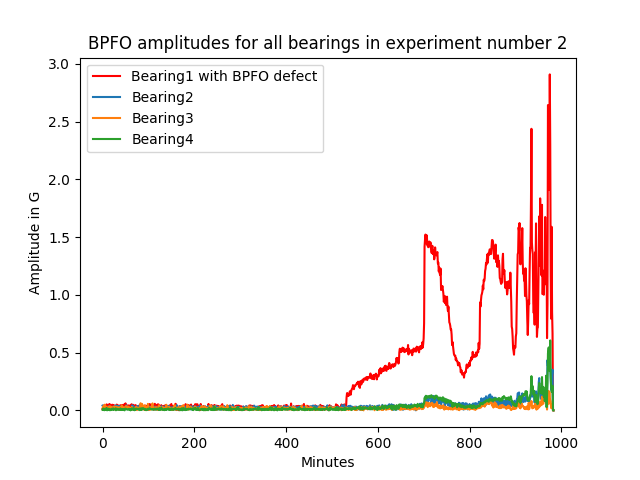
\includegraphics[width=4in]{../fig/experiment2_bearing_fft_amp.png}
		% 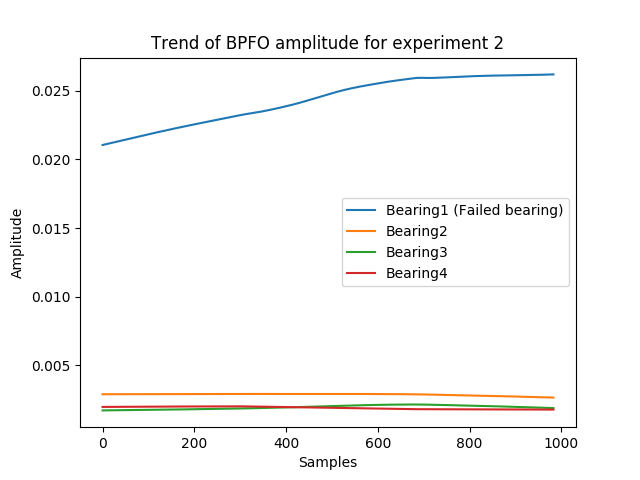
\includegraphics[width=4.4in]{../fig/experiment2_bearing_fft_trend.png} 
		\caption{BPFO amplitude evolution for all bearinags over time}
		\label{fig:dq1}
	\end{figure}
%	Here, you may discuss your findings based on your results, their strengths and limitations. 
%	Note that this discussion is more high level than discussions made in relation to results you have achieved and presented in the previous chapter. 
%	The discussion here should put your work in larger context. 
%	You may address if you achieved what you had intended to do, why not (if you did not), if you got results in which you did not expect, why the results are important, why there are limitations in using the results, or if there are opportunities to transfer your results and findings into other domains, and so on.
	%%=========================================
	\section{Recommendations for Further Work}
	\label{sec:recommendations_for_further_work}
	
	
	The recommendations may be classified as:
	\begin{itemize}
		\item Short-term
		\item Medium-term
		\item Long-term
	\end{itemize}
	
\end{document}
